\section{Introduction}
    Trying to outline the objectives and goals of this paper. A `Short' treatment of trust and its definitions. Address the definition that we are interested (human-autonomy interaction). Discuss different fields that are interested in trust. Review mechanisms that are used in each field. Propose introspection as the set of all of the used methods, plus those that are missing.
    
    Introduces the idea of trust (and references some of the work in this area). This paper introduces a topic called \emph{circumspection of artificial agents}, which is defined as agents that produce the tools to be circumspective. Or in other words they possess the tools to be \emph{introspective} and \emph{extrospective}. Highlights how circumspective tools are necessary for human-agent trust relationships. It highlights the work that has already been done in many other research fields, which is knows by other names and descriptions, and shows that they all have common themes.

    Some ideas for content:

    \begin{itemize}[htbp]
        \item Introduce trust, with a bias towards non-interhuman trust (i.e. human-computer, human-robot, human-machine)
        \item List some of the fields that are interested in circumspection (even if they don't know it yet), give examples of why
        \item break down other fields into different AI capabilities. This will help outline different assurances for different purposes.
    \end{itemize}

    Define Trust-Related Behaviors (TRBs) up here somewhere.
\subsection{Artifically Intelligent Agents}
    An Artificial General Intelligence (AGI) possess all capabilities shown in Figure \ref{fig:AIcapabilities} (as the typical human does). At this time we do not have the ability to build AGIs, instead we design highly specialized versions which will be referred to as AIs in this paper. An AI is an agent that possess, to some extent, at least one of the capabilities shown in the figure. This is a very weak notion of AI, but encompasses much of the current systems that are being marketed as artificially intelligent.

    The field called machine learning (ML) is a piece of the AI research landscape. Individual ML algorithms might be thought of as being a highly specialized AI that is contained within only one of the AGI capabilities.

	\begin{figure}[htbp]
    	\centering
     	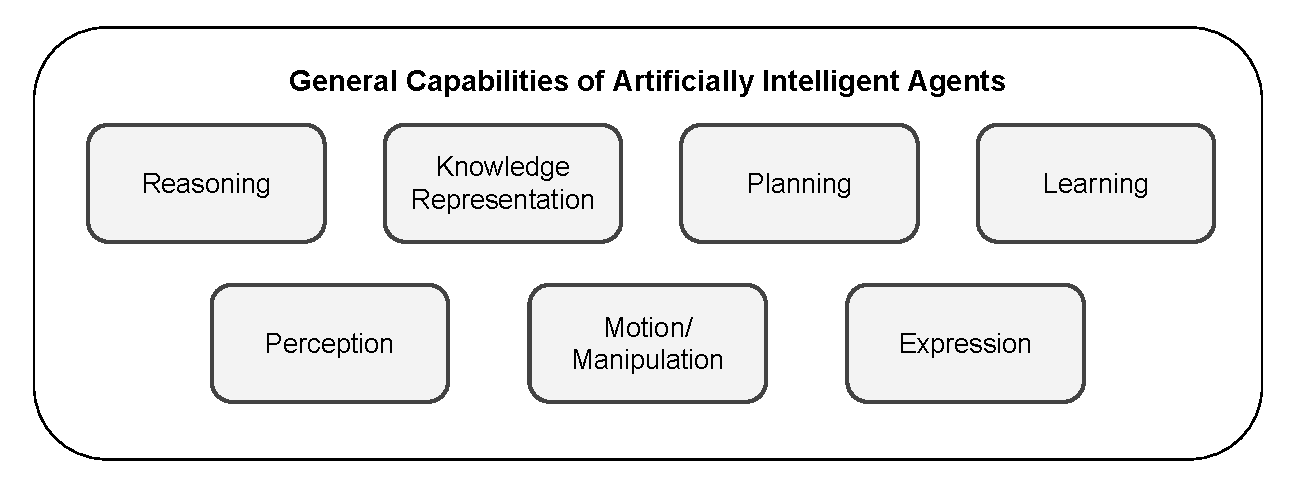
\includegraphics[width=0.9\textwidth]{Figures/AI_capabilities}
    	\caption{List of the capabilities of an artificial general intelligence. In this paper an AI is defined as a system that possesses at least one of the capabilities illustrated. \textbf{The Social Intelligence and Creativity capabilities are not going to be considered in this paper\ldots add something further about that}}
        \label{fig:AIcapabilities}
    \end{figure}

    Here are a few examples an unmanned aerial system (UAS) might possess the following capabilities: Planning, Perception,  and Motion/Manipulation. A personal assistant might be capable of Interaction, Learning, and Reasoning. An image classifier might possess the capability to learn image classes from labeled examples and predict the class of never-before-seen new images.
    

\section{The Case for Human-AI Trust}
    Trust is a subject that has been extensively studied in many different disciplines. something, something \ldots.

    In the era of the internet there was a surge of interest in trust due to the appearance of e-commerce. Suddenly, the internet became a new forum for buying and selling wares and services. But building relationships of trust between consumers and vendors was critical to the success of using the internet as a tool for commerce. This survey will not exhaustively review the literature on trust those interested might refer to the following works by \citet{McKnight2001-fa}, and \citet{Lewicki2006-hj}.

    Due to wide interest spanning many disciplines it is difficult, if not impossible, to write a succinct definition that would appease all interested parties. In their work relating to e-commerce \citet{McKnight2001-fa} reviewed much of the existing trust literature and attempted to distill the main concepts into a trust model that spanned disciplines. That model is shown, with some minor adaptations, in Figure \ref{fig:UserTrust}.

	\begin{figure}[htbp]
    	\centering
     	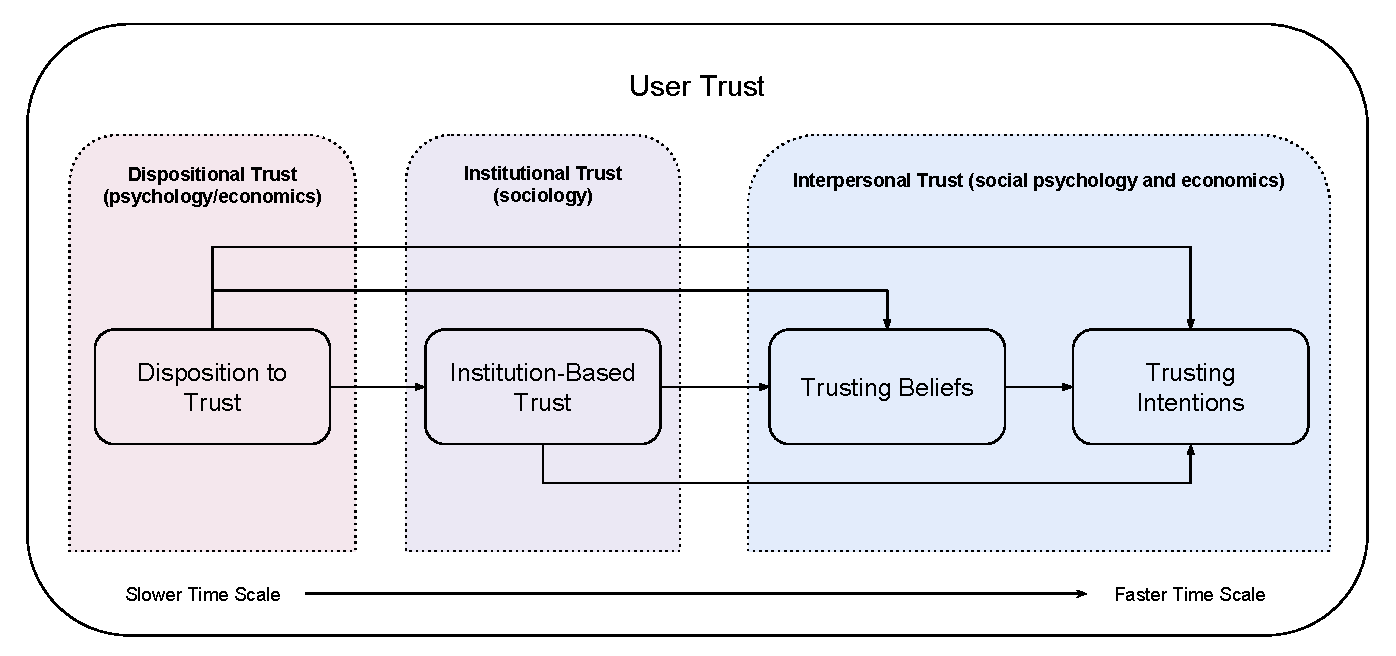
\includegraphics[width=0.9\textwidth]{Figures/UserTrust}
    	\caption{Interdisciplinary trust model proposed by \citet{McKnight2001-fa}. The three main categories are delineated and corresponding disciplines that are interested are listed withing parentheses. }
        \label{fig:UserTrust}
    \end{figure}

    Each of the three main subcategorie

    Trust results in some kind of behavior, which \citet{McKnight2001-fa} calls `trust-related behaviors' (TRBs). In the case of a human-autonomy relationship examples of TRBs might be the kinds of tasks the human user assigns to the autonomy, or whether the human will use a plan produced by the autonomy.

\section{Calibration of TRBs}
    As yet trust is not a quantity that can be directly measured. Rather, its relative magnitude must be observed through changes in TRBs. \citet{Parasuraman1997-co} were interested in understanding the use of automation which they defined as ``\ldots the execution by a machine agent (usually a computer) of a function that was previously carried out by a human''. Within this scope they define the following terms: a) \emph{misuse}, the overreliance on automation, b) \emph{disuse}, the underutilization of automation, and c) \emph{abuse}, inappropriate application of automation.

    It is proposed that, analogously, the definitions of \emph{misuse}, \emph{disuse}, and \emph{abuse} can apply to the relationship between humans and autonomy (where autonomy is defined as a system, such as an artificial agent with processing power possibly located on a physical robot, that is able to independently act in uncertain environments to accomplish a goal).
    
    To be more formal, let the total set of TRBs as $\mathcal{T}$. Then as subsets of $\mathcal{T}$ define the set of misue actions as $\mathcal{M}$, the set of disuse actions as $\mathcal{D}$, and the set of abuse actions as $\mathcal{A}$. Next, define the total set of innapropriate TRBs $\mathcal{I}$ as the union of $\mathcal{I} = \mathcal{M}\cup \mathcal{D}\cup\mathcal{A}$. Having defined the set of inappropriate actions, the set of appropriate TRBs can be defined as $\mathcal{U}$ as the compliment of the set of inappropriate TRBs $\mathcal{U} = \mathcal{I}^\prime$. This is illustrated in Figure \ref{fig:appropriate_use}, where the set of appropriate actions $\mathcal{U}$ is the gray colored area (i.e. all TRBs \emph{not} in either of the three sets of inappropriate TRBs).
    
	\begin{figure}[htbp]
    	\centering
     	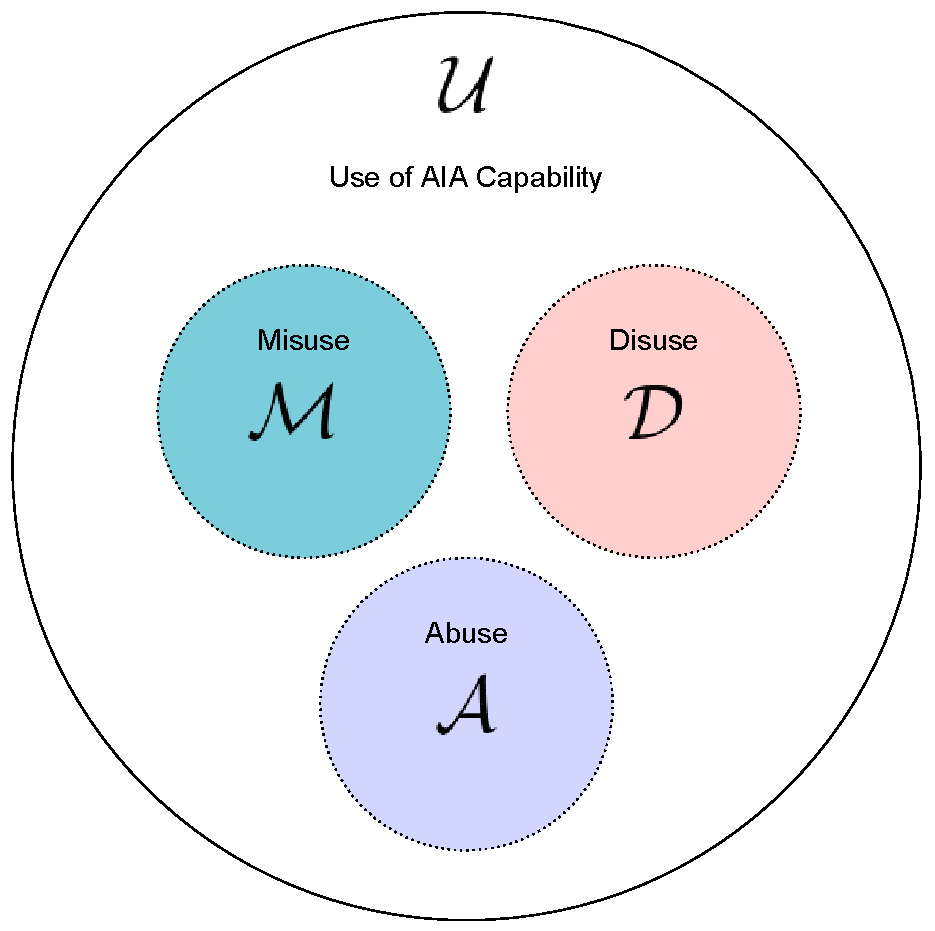
\includegraphics[width=0.6\textwidth]{Figures/misuse_disuse_abuse}
    	\caption{Graphic representing the total space of user actions, in which the inappropriate uses $\mathcal{M}$, $\mathcal{D}$, and $\mathcal{A}$ lie. The set of inappropriate uses $\mathcal{I}$ is the union of $\mathcal{M}$, $\mathcal{D}$, and $\mathcal{A}$. The appropriate set of actions $\mathcal{U}$ is the compliment of \mathcal{I}, or the part of $\mathcal{T}$ that does not include $\mathcal{I}$.}
        \label{fig:appropriate_use}
    \end{figure}
    
    In order to ensure that humans use autonomous systems appropriately it is critical that the user trust be calibrated to elicit behaviors that are within $\mathcal{U}$.

    A simple feedback loop, as illustrated in Figure \ref{fig:SimpleTrust} will allow the AI to calibrate the TRBs of the user by providing assurances.

	\begin{figure}[htbp]
    	\centering
     	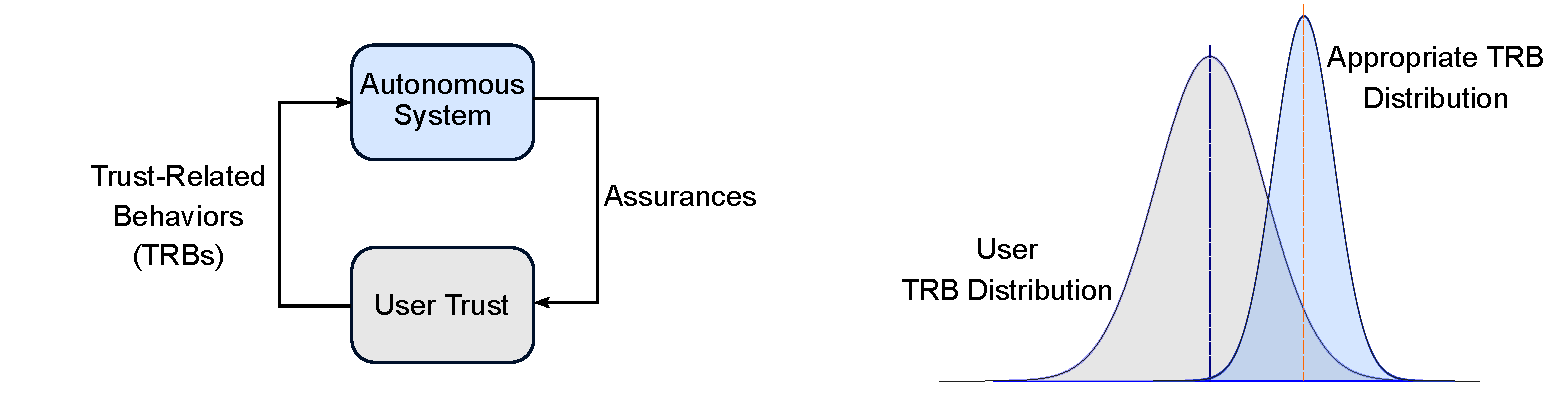
\includegraphics[width=0.6\textwidth]{Figures/SimpleTrust}
    	\caption{Simple Feedback loop that allows an AI to influence User Trust in order to calibrate the TRBs. The right side shows an example user TRB distribution and the appropriate TRB distribution. Calibrating TRBs involves making the two distributions as similar as possible.}
        \label{fig:SimpleTrust}
    \end{figure}

\section{Who cares?}
    Because everyone wants to trust their AIs, whether that be a single classification or regression algorithm, or a more interactive personal assistant that can understand language and communicate. Everyone wants to know how to trust these systems.  

    \paragraph{Why lay out AGI, when it doesn't exist yet?} Because this architecture is supposed to illustrate how the entire spectrum of AI from a single ML algorithm to an autonomous vehicle, to a full AGI operate on very similar grounds. That is that 

	\begin{sidewaysfigure}[htbp]
        \centering
    	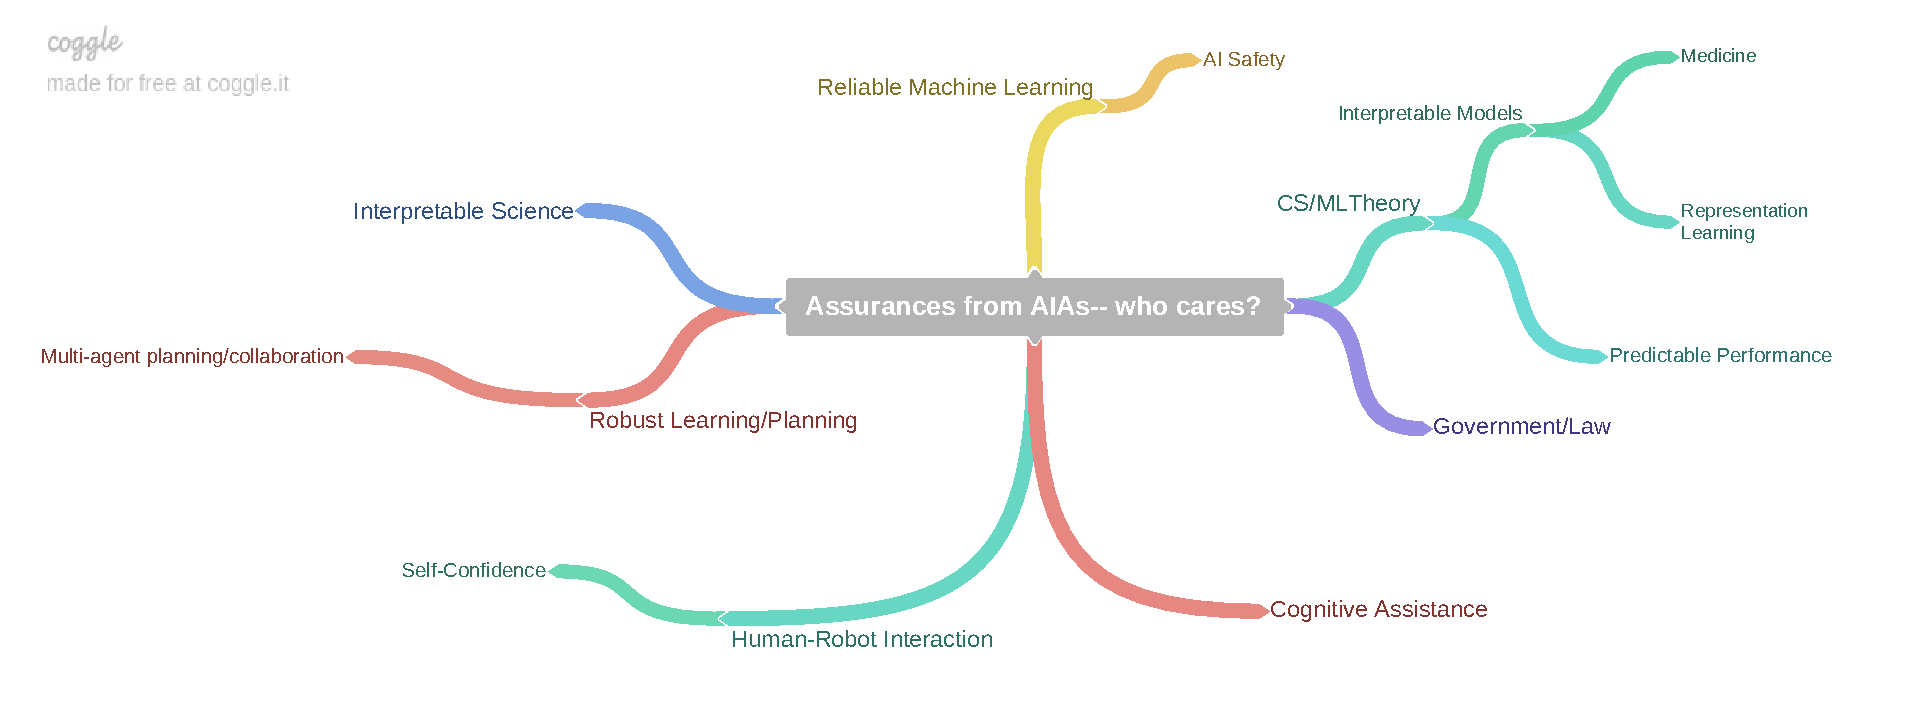
\includegraphics[width=8in]{Figures/WhoCares}
    	\caption{A diagram showing some of the academic disciplines that want to trust AIs more fully}
        \label{fig:WhoCares}
    \end{sidewaysfigure}

    \paragraph{Science} Talk about why the science discplines care
    \paragraph{Robust Learning/Planning}
    \paragraph{HRI}
    \paragraph{Cognitive Assistance} 
    \paragraph{Government/Law} Regulations on the interpretability of certain algorithms, usage for assistants to lawyers.

    \textbf{Perhaps a table showing the field vs. the AI capability?}, this would help to illustrate the varying needs by fields. Perhaps highlight oversights?

    \textbf{Perhaps a table showing the 

\section{Methodology}
    In this paper I am focusing on a human-autonomy relationship between a single human user (User), and a single autonomous system (Autonomy). Furthermore, I will only be considering a one-way trust relationship, that is that the autonomy has perfect trust towards a user and that trust does not change with time. 

    here are the assumptions:

    \begin{itemize}
        \item 1:1 relationship (i.e. not groups)
        \item Focus on Belief and Behavior classes (faster time scale)
        \item Autonomy is honest and friendly
        \item others \ldots
        \item assume that the AI has a better idea of true distribution than the user (AI, may also need to learn with experience)
    \end{itemize}


\section{Conclusion}
    Revisit the key ideas of the paper:

    \begin{itemize}
        \item trust is a key factor for human-agent interaction
        \item many fields care about it
        \item circumspection is a common framework
        \item circumspection has several key properties that encompass the different research fields
    \end{itemize}

\newpage
